%%%%%%%%%%%%%%%%%%%%%%%%%%%%%%%%%%%%%%%%%%%%%%%%%%%%%%%%%%%%%%%%%%%%%%%%%%%%%%%%
% This is the Mamba3D user manual Tex source

\documentclass[a4paper,10pt,oneside]{article}
\usepackage[table]{xcolor}
\usepackage{mamba}

\title{Mamba 3D User Manual}
\author{Nicolas BEUCHER}
\date{\today}

%%%%%%%%%%%%%%%%%%%%%%%%%%%%%%%%%%%%%%%%%%%%%%%%%%%%%%%%%%%%%%%%%%%%%%%%%%%%%%%%
% Tip and warning boxes environments
\definecolor{lightblue}{RGB}{220,220,255}
\newenvironment{tipBox}
{
    \begin{center}
    \begin{tabular}{ | b{0.1\textwidth} b{0.8\textwidth} | }
    \hline
    \rowcolor{lightblue}
    
\includegraphics[width=0.1\textwidth]{Crystal_Clear_action_info.png} &
}
{
    \\
    \hline
    \end{tabular}
    \end{center}
}

\newenvironment{warnBox}
{
    \begin{center}
    \begin{tabular}{ | b{0.1\textwidth} b{0.8\textwidth} | }
    \hline
    \rowcolor{yellow}
    
\includegraphics[width=0.1\textwidth]{Crystal_Clear_app_error.png} &
}
{
    \\
    \hline
    \end{tabular}
    \end{center}
}

%%%%%%%%%%%%%%%%%%%%%%%%%%%%%%%%%%%%%%%%%%%%%%%%%%%%%%%%%%%%%%%%%%%%%%%%%%%%%%%%
% Document

\begin{document}

\mambaCover
\mambaContent

\section{Introduction}

Not all images are in two dimensions ! However Mamba works only with basic 2D
images and that's sad...

Mamba3D was created to correct this most regrettable fact. For surely,
mathematical morphology tools, that present powerful and elegant tools to 
perform image analysis in 2D, will allow miracles in 3D, right ? 

Well we can't answer this for you. However, while creating and trying the first
version of Mamba3D, we learned some wisdoms (like adding a dimension is not
as straighforward as it might seem) about 3D images that we wish to
impart with you along with the best way to use Mamba3D.

We also would like to remind you that Mamba3D is still young and may lack
some operators or capabilities that you would like to have.

\pagebreak

\section{License}
\label{cha:License}

Here is a copy of the license of Mamba3D. This license is known as the X11 license
(also named MIT license). This is similar to the Mamba license.

\vspace{0.5cm}

\begin{minipage}[c]{0.8\textwidth}%
 {\small Copyright (c) <2011>, <Nicolas BEUCHER and ARMINES for the Centre de 
 Morphologie Math\'{e}matique(CMM), common research center to ARMINES and MINES 
 Paristech>}{\small \vspace{0.5cm} \par}

{\small Permission is hereby granted, free of charge, to any person
obtaining a copy of this software and associated documentation files
(the \textquotedbl{}Software\textquotedbl{}), to deal in the Software
without restriction, including without limitation the rights to use,
copy, modify, merge, publish, distribute, sublicense, and/or sell
copies of the Software, and to permit persons to whom the Software
is furnished to do so, subject to the following conditions: The above
copyright notice and this permission notice shall be included in all
copies or substantial portions of the Software.}{\small \vspace{0.5cm} \par}

{\small Except as contained in this notice, the names of the above copyright 
holders shall not be used in advertising or otherwise to promote the sale, use 
or other dealings in this Software without their prior written authorization.}
{\small \vspace{0.5cm} \par}

{\small THE SOFTWARE IS PROVIDED \textquotedbl{}AS IS\textquotedbl{},
WITHOUT WARRANTY OF ANY KIND, EXPRESS OR IMPLIED, INCLUDING BUT NOT
LIMITED TO THE WARRANTIES OF MERCHANTABILITY, FITNESS FOR A PARTICULAR
PURPOSE AND NONINFRINGEMENT. IN NO EVENT SHALL THE AUTHORS OR COPYRIGHT
HOLDERS BE LIABLE FOR ANY CLAIM, DAMAGES OR OTHER LIABILITY, WHETHER
IN AN ACTION OF CONTRACT, TORT OR OTHERWISE, ARISING FROM, OUT OF
OR IN CONNECTION WITH THE SOFTWARE OR THE USE OR OTHER DEALINGS IN
THE SOFTWARE. }%
\vspace{1cm}
\end{minipage}

\begin{warnBox}
Please note that this license does \textbf{\textsc{not}} cover documentation and
images found in source packages.
\end{warnBox}

\pagebreak

\section{Requirements}
\label{cha:Requirements}

To use Mamba3D, you will need:
\begin{itemize}
\item A compatible version of Mamba installed on your computer. Compatibility
information may be found on the website \url{http://www.mamba-image.org/}.
\item VTK (see \url{http://www.vtk.org/} for more info) with python bindings
if you want to use the integrated display. In particular Mamba3D uses VTK
functions to bind the 3D display to Tkinter. Appendix \ref{cha:vtkInst}
describes the compilation and installation instruction to create a python
module for VTK on Windows.
\end{itemize}

\begin{tipBox}
While Mamba3D will certainly work on a large range of systems, it is still
strongly recommanded that you work on a powerful computer if you want an
optimal experience with it (see section \ref{cha:perfo} for more information).
\end{tipBox}

To compile or modify the sources, you will need:
\begin{itemize}
\item Python version 2.6 or later with the distutils package.
\item Python development headers (normally comes with Python on Windows systems 
but you may need to install them on Linux systems).
\item SWIG version 1.3.33 or later.
\item GCC version 4.3.0 or later (or its Windows version MinGW32).
\item  Under Windows, you may choose Microsoft Visual C++ Express 2008 (to 
compile you will then need the stdint.h header. You can find it at 
\url{http://msinttypes.googlecode.com/svn/trunk/stdint.h}. Copy it in the VC/include 
directory of your Visual C++ installation).
\end{itemize}
Compilation instructions are given in the next section.

\pagebreak

\section{Installation/compilation}
\label{cha:Inst}

Mamba3D can be compiled and installed on various platforms and systems.
The compilation, distribution and installation are performed using the
distutils package which is the standard Python way to do it
(see \url{http://docs.python.org/library/distutils.html}).

If you are using a Windows system, you can use the provided installer. Grab it
at the website, launch it and follow the instructions.

To compile, make sure you have correctly installed the required tools (see section
\ref{cha:Requirements}) and that they appear in your PATH environment variable.
In particular, make sure that SWIG binary (swig.exe) and GCC binary (gcc.exe)
paths are devoid of spaces as this may cause problems to the setup script.

\begin{enumerate}
\item Get the latest version of the source (package "Mamba.X.X.zip")
\item Extract it in your local directory
\item Open a command line window
\item Browse to the created directory "Mamba.X.X"
\item Browse to src/mambaAddons/mamba3D
\item type:

\texttt{python setup3D.py build\_ext build} (All systems)

\item You can then install it.

\texttt{python setup3D.py install}

\end{enumerate}

Alternatively, on Windows, you can create the installer that will allow you to 
distribute more easily your own version of Mamba3D. Replace step 6 above by the 
following instruction:

\begin{enumerate}
\setcounter{enumi}{5}
\item type:

\texttt{python setup3D.py build\_ext bdist\_wininst} (Windows only)

\end{enumerate}

The installer produced will be in the dist directory.

You can found some complements regarding compilation and installation in
appendix \ref{cha:vtkInst}.

\pagebreak

\section{Using Mamba3D}
\label{cha:Use3D}

In this section, we will describe how Mamba3D works and how to use it
efficiently. We will also address some problems or difficulties you may
encounter

\subsection{Mamba3D philosophy}

Mamba3D was created to be able to apply the same algorithms developped for
2D images using Mamba to 3D images. To achieve this goal, several choices
were made:

\begin{itemize}
\item Reuse as much as possible the basic C operators from Mamba to perform
the 3D computations to avoid rewriting them (Apart from hierarchical and
labelling operators this was actually possible).
\item Make sure functions and classes keep the same "look and feel" as their
counterpart in Mamba.
\item Provide an adapted display as there is one in Mamba.
\end{itemize}

These choices had consequences on the design of the package and thus on its
capacities. Overall we believe the possible downfall of that choices are
dimmed by the gains in terms of easiness of use, reuse of proven and robust
code and work versus objective ratio.

\subsection{Importing the package}

To use Mamba3D, simply type in your Python console:

\lstset{language=Python}
\begin{lstlisting}
import mamba3D
\end{lstlisting}

This is the recommended Python import method because it separates each module
you may use in its own name reference space. However this is quite painful
to work with when you are using Mamba3D in a console mode as all the function 
calls have to be preceded by:

\lstset{language=Python}
\begin{lstlisting}
mamba3D.
\end{lstlisting}

So to avoid this, type:

\lstset{language=Python}
\begin{lstlisting}
from mamba3D import *
\end{lstlisting}

\subsection{Creating and manipulating 3D images}

The basic data model used in Mamba3D is the image3DMb image class.

This class is derived from the sequenceMb class in the mambaComposed package.
You should know that this class is actually a stack of standard Mamba images
(imageMb object) with all the same size and depth. The dimension of a 3D image
is thus given by the size of the mamba images inside the stack and by its
length. This choice may seem strange because it differentiates one direction
(supposedly z-axis) in the data structure from the other two (x-axis and
y-axis) but it was dictated by the need to reuse as much as possible the 
basic C functions of Mamba which work with imageMb low-level structure.

There is a wide range of possibilities to create a 3D image object :
\begin{itemize}
\item \texttt{\textbf{image3DMb()}} : without arguments will create an empty
greyscale 3D image (by default its size is 256x256x256).
\item \texttt{\textbf{image3DMb(im3D)}} : will create a 3D image using the
same width, height, length and depth than 3D image 'im3D'.
\item \texttt{\textbf{image3DMb(im)}} : will create a 3D image using the same
width, height and depth than 2D image 'im' (a imageMb object). Its
lenght will be defaulted to 256.
\item \texttt{\textbf{image3DMb(depth)}} : will create a 3D image with the
desired 'depth' (1, 8 or 32) and default size (256x256x256).
\item \texttt{\textbf{image3DMb(path)}} : will load the image sequence located
in 'path', see the load method.
\item \texttt{\textbf{image3DMb(im3D, depth)}} : will create a 3D image using
the same size than 3D image 'im3D' and the specified 'depth'.
\item \texttt{\textbf{image3DMb(im, length)}} : will create a sequence using
the same width, height and depth than 2D image 'im' (a imageMb object). Its
length will be the specified 'length'.
\item \texttt{\textbf{image3DMb(path, depth)}} : will load the image sequence
located in 'path' and convert it to the specified 'depth'.
\item \texttt{\textbf{image3DMb(width, height, length)}} : will create a 
greyscale 3D image with 'width', 'height' and 'length'.
\item \texttt{\textbf{image3DMb(width, height, length, depth)}} : will create
a 3D image with the given parameters.
\end{itemize}

Refer to the Python reference manual of Mamba to get more info about the 
sequenceMb class. Specific 3D image methods information can be found in the
Mamba3D Python reference. In particular, image3DMb class defines a method
to load raw 3D data.

\subsection{Displaying images}
\label{cha:disp_im}

As for basic Mamba images, 3D images can be displayed each individually with
their own window, see figure \ref{fig:dis_base}. Mamba3D offers by default
two possibilities to display 3D images and enables you to define your own
display. Mamba3D allows you to active multiple displays for one image.

\begin{tipBox}
The foot data used for the display demo in this section can be found at
\url{http://tc18.liris.cnrs.fr/code_data_set/3D_images.html}
\end{tipBox}

\subsubsection{Volume rendering display}
This display is ensured through the VTK library. This is the default display
if you have VTK (with Python bindings) installed on your computer.

To activate the volume display, type:

\lstset{language=Python}
\begin{lstlisting}
# Shows the 3D image in its own window
im3D.showDisplay()
# The previous call worked because VTK is the default display method
# you can explicitly ask for it
im3D.showDisplay("VTK")
\end{lstlisting}

\begin{figure}
\centering
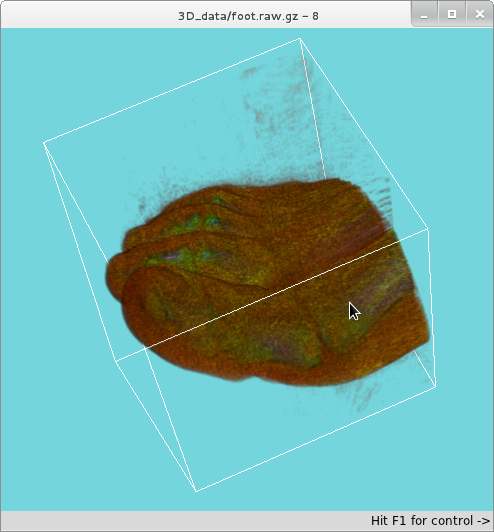
\includegraphics[scale=0.5]{display_base.png}
\caption{Image volume displayer window}
\label{fig:dis_base}
\end{figure}

The image is displayed inside its bounding cube and you can control its rotation
and zoom with your mouse.

The display comes with an integrated controller which allows you to change
the various options of display available. As shown in figure \ref{fig:dis_ctrl},
you can change the opacity, the background color and the rendering methods.

The transparency/opacity of a pixel depends on its value. By clicking on the 
transparency bar, every pixel with value below will be transparent and above
pixels will be opaque. You can also change the opacity by calling the 
appropriate method:

\lstset{language=Python}
\begin{lstlisting}
# Sets the opacity in reverse of default opacity (but let value 0 stay 
# fully transparent)
l = range(255,-1,-1)
l[0] = 0
im3D.setOpacity(l)

# Resetting the opacity to its default value
im3D.resetOpacity().
\end{lstlisting}

The color transfer function works the same as for the mamba images. In fact, you
must call the same method with the same kind of parameters.

\lstset{language=Python}
\begin{lstlisting}
# Indicates that im3D will use palette as a color transfer function
im3D.setPalette(palette)

# Resets any palette conversion (the image will return to greyscale display)
im3D.resetPalette()
\end{lstlisting}

To change the background, just click on the background bar. It will open a
color chooser dialog box in which you can pick up any background color you
might want.

\begin{figure}
\centering
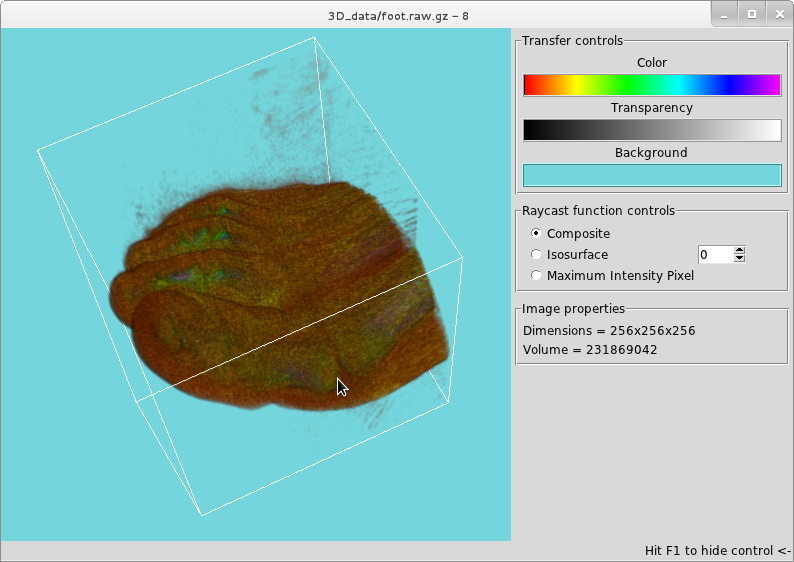
\includegraphics[scale=0.5]{display_ctrl.png}
\caption{Volume display controls}
\label{fig:dis_ctrl}
\end{figure}

Mamba 3D uses volume rendering techniques to display the data. VTK provides
three distinctive methods to perform volume rendering :
\begin{itemize}
\item \textbf{Composite} : the result is a blend of all the pixels crossed by
the ray of light accordingly to their color and transparency.
\item \textbf{Isosurface} : the result shows only pixels with a given
value. It also use shading to allow a better visualisation of the volume.
\item \textbf{Maximum Intensity Pixel (MIP)} : the result is the color and
transparency of the pixel with the highest value that the light ray hit.
\end{itemize}
You can see the results of the 3 different methods in figure 
\ref{fig:dis_method}.

\begin{figure}
\centering
\begin{tabular}{ccc}
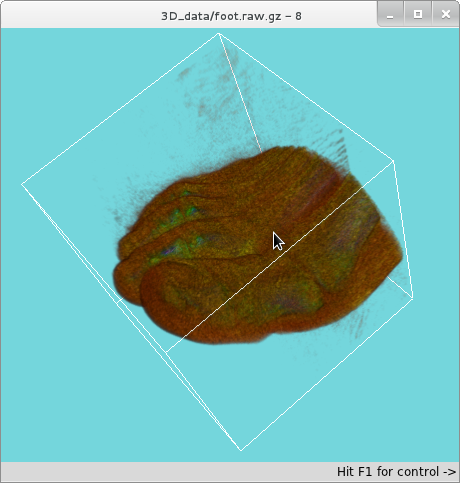
\includegraphics[width=0.25\textwidth]{display_compo.png} & 
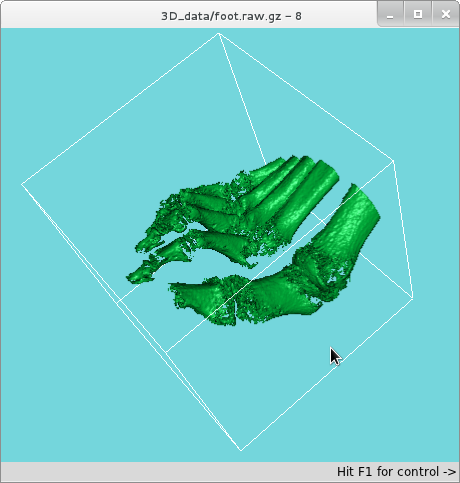
\includegraphics[width=0.25\textwidth]{display_isosurface.png} &
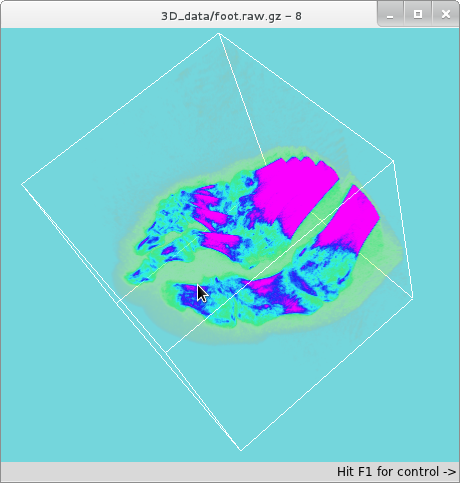
\includegraphics[width=0.25\textwidth]{display_mip.png} \\ 
Composite &
Isosurface &
MIP \\ 
\end{tabular}
\caption{Volume rendering techniques}
\label{fig:dis_method}
\end{figure}

You can rotate (holding your mouse left button while moving it), zoom in and
out (same movement while holding the right button) and displace the image
(this time by holding both the left button and the shift key on your keyboard
while moving the mouse). This allows you to view more precisely any area of
your image. You can restore the initial settings by pressing r (Although this
does not seem to affect rotation).

We feel this display is appropriate to get an overall idea of your
result. However, it may lack precision and it could be troublesome to
understand what or where you are looking at. Use it cautiously.

\subsubsection{Projection display}
This display is basically an adaptation of the 2D display available in Mamba.
It is a basic plane projection along the three axis.

To activate the volume display, type:

\lstset{language=Python}
\begin{lstlisting}
# Shows the 3D image in its own window using projection along axis
# Note that if you have opened a VTK display this new one will not
# replace it (you will now have 2 displays available).
im3D.showDisplay("PROJECTION")
\end{lstlisting}

\begin{figure}
\centering
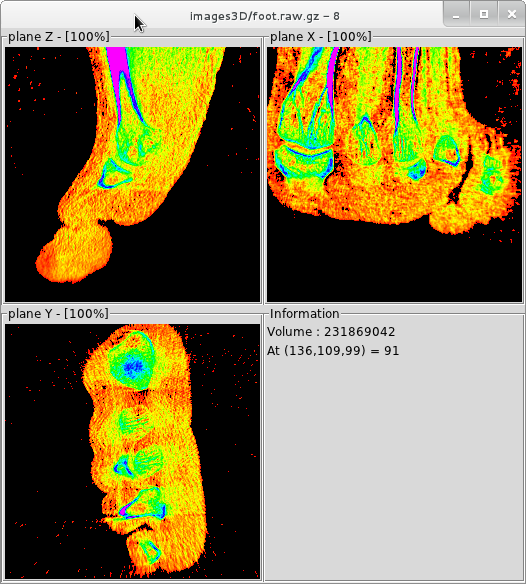
\includegraphics[scale=0.5]{display_proj.png}
\caption{Image projection displayer window}
\label{fig:dis_base}
\end{figure}

You can navigate through planes moving your mouse while holding <ctrl> down.
The mouse motion will allow you to change the plane following it (the displayer
shows a red cross to indicate where you are in the image data).

This display does not support opacity tuning. However you can use a color
palette (same procedure that for VTK display).

This is a more appropriate display if you need precision and careful
analysis of a result. However it only shows a limited amount of the
image at any given time.

\subsubsection{3D displays particularities}
As you will see, unlike 2D images displays that are updated as the computations
progress, 3D images displays are not (for performance reasons). You will have
to update them manually by either hitting key <F5> on your keyboard (with
the focus on the display you want to update) or call the appropriate method
when you need an update:

\lstset{language=Python}
\begin{lstlisting}
# Updates the display
im3D.updateDisplay()
\end{lstlisting}

We tried to provide Mamba3D with a coherent, useful and appropriate display.
However, contrary to 2D images, 3D images are difficult to represent on a 2D
display. Be sure to correctly configure the display before analysing results.
We do not believe Mamba3D display will fit all situations and you are
encouraged to look at other possible ways to display your data if you
think the one in Mamba3D in not good for you (refer to section \ref{cha:create_disp}
to get an idea of how to create your own display and use it).

Lastly, as 3D images in Mamba3D are stacks of 2D images (imageMb objects) you 
always have the possibility to activate their own display at all time.

\lstset{language=Python}
\begin{lstlisting}
# Activates the display for slice number 128 of 3D image
im3D[128].showDisplay()
\end{lstlisting}

\subsection{Grids and structuring elements}

Mamba3D defines various grids and structuring elements with them. You will
find they work the same as in Mamba except that they are a bit more
difficult to represent. We tried in this section to give you an overview
of what they look like. Also they have some limitations that we think you
should be aware of.

As a foreword, we would like to explain how 3D grids are built in Mamba3D.
Instead of Mamba, where grids where defined for low-level C operators, Mamba3D
grids are very high level complex structures. They are built using 2D grids and
a mix of programmation magic. Some operators were rewritten in low-level C
functions working on 3D images because their 2D counterpart could not be adapted
to a 3D structure (e.g. hierarchical queues operators). As they work using the
grid, we defined some grids in low-level C but not all of them (too much work).
So some operators may not work with the grid you selected. Be warned !

\begin{tipBox}
Grids in Mamba3D are strongly influenced by crystallography. For example,
the face centered cubic grid is describing the way carbon atoms are 
crystallized to form diamonds and centered cubic (also named body centered
cubic) is a structure by which iron atoms organise themselves. Of course, there
is a lot of other structures in crystals that are not represented in Mamba3D.
\end{tipBox}

Mamba3D defines 3 grids (the figures representing the grids are projections,
they indicates directions/neighbors numbers):

\begin{itemize}
\item \textbf{CUBIC}: The very basic cubic grid, built by stacking square
grids one on the other. See figure \ref{fig:cubic_grid}.

\begin{figure}
\centering
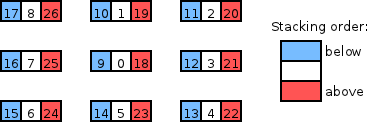
\includegraphics[width=0.55\textwidth]{cubic_grid.png}
\caption{Cubic grid}
\label{fig:cubic_grid}
\end{figure}

\item \textbf{FACE\_CENTER\_CUBIC}: A face centered cubic grid. It is in fact
built by stacking hexagonal grids one on the other with a slight shift. See
figure \ref{fig:fcc_grid}.

\begin{figure}
\centering
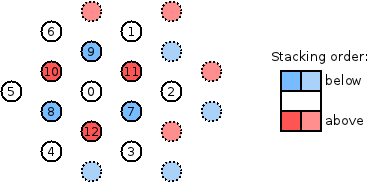
\includegraphics[width=0.55\textwidth]{fcc_grid.png}
\caption{Face centered cubic grid}
\label{fig:fcc_grid}
\end{figure}

\item \textbf{CENTER\_CUBIC}: Known as the body centered cubic, this grid is
built by stacking square grids with a half shift in the two directions. See
figure \ref{fig:ccubic_grid}. This grid is not supported by low-level C
operators.

\begin{figure}
\centering
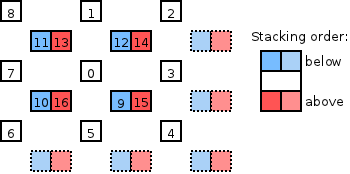
\includegraphics[width=0.55\textwidth]{ccubic_grid.png}
\caption{Centered cubic grid}
\label{fig:ccubic_grid}
\end{figure}

\end{itemize}

As it is, we could have added a lot more grids in Mamba3D. For example,
we could have built a grid stacking without any shifted hexagonal grids.
We chose not to do it, but it does not mean you can't, although we doubt very
much you find such grids useful. In this event, we encourage you to look
at section \ref{cha:create_grid}.

Regarding the FACE\_CENTER\_CUBIC, you can notice on figure \ref{fig:fcc_grid}
that the triangles drawn by below directions (blue) and above directions (red)
do not point the same way. This is very important to be able to draw a 
cuboctahedron instead of an anti-cuboctahedron.

On top of these grids we can now build structuring elements just like we did
in Mamba. We predefined four structuring elements in Mamba3D:

\begin{itemize}
\item \textbf{CUBIC3X3X3} : A three pixels large cube. Based on the CUBIC grid.
\item \textbf{CUBIC2X2X2} : A two pixels large cube. Based on the CUBIC grid.
\item \textbf{CUBOCTAHEDRON} : A cuboctahedron. Based on the
FACE\_CENTER\_CUBIC grid.
\item \textbf{CUBOCTAHEDRON\_BIS} : Another cuboctahedron. Based on the
CENTER\_CUBIC grid. This one is slighty rotated.
\end{itemize}

You can also, of course, create your own structuring elements:

\lstset{language=Python}
\begin{lstlisting}
# Creating a small pyramid
pyramid = structuringElement3D([0,1,2,3,14], CENTER_CUBIC)

# Why not a tetrahedron
tetrahedron = structuringElement3D([0,1,2,11], FACE_CENTER_CUBIC)

# You can of course build pyramids and tetrahedrons with
# different directions. The next two are a bit better because they
# are centered
pyramid2 = structuringElement3D([0,9,10,11,12], CENTER_CUBIC)
tetrahedron2 = structuringElement3D([0,7,8,9], FACE_CENTER_CUBIC)
\end{lstlisting}

\subsection{Computations/Functions}

Performing computations with Mamba3D was meant to be as close as possible
as the way they are done in Mamba. Thus function names are identical except
for a postfix "3D" indicator.

\lstset{language=Python}
\begin{lstlisting}
# For example the erode function in Mamba
erode(imIn, imOut, n=1, se=DEFAULT_SE, edge=FILLED)
# will become in Mamba3D (beware of the mamba.FILLED needed if you did 
# not import mamba)
erode3D(imIn, imOut, n=1, se=CUBOCTAHEDRON, edge=mamba.FILLED)
\end{lstlisting}

Although it might seem bothersome to add the "3D" postfix to every
function you are using when computing in 3D, it is also needed to be able to
use both the 2D functions and their 3D counterpart in the same script.

This naming convention was also adopted, for the most part, by module
names in the Mamba3D package.

As simple as it is, you will still face difficulties if you try to translate
your 2D algorithm into 3D. First, computations take more time (see section
\ref{cha:perfo}) but Mamba3D does not offer all the functions found in
the Mamba API. The section \ref{cha:missing} describes some of the 
main differences between the two.

\subsection{Performance discussion}
\label{cha:perfo}

Performing computation on 3D data is performance consuming. For example, if
you compare a 2D erosion with a hexagonal structuring element versus a 3D
erosion using a cuboctahedron structuring element, you will have to perform
twice more operations per pixel in the later. If you take into account that
the number of pixels is also greater in 3D (and not by a small amount), you end
up with a very large difference of speed between the two operations.

Thus, if you need to process 3D images, you get only three choices, get patient, 
get a faster computer or code a library fully optimized for 3D operations 
(which Mamba3D isn't).

Another performance problem arises with the display. VTK is a very powerful
library offering state of the art methods and algorithms to display 
data of all kinds. Mamba3D uses the volume rendering techniques based on 
\textbf{CPU computation and not GPU} implemented into VTK. Of course, they
are slower than the ones using the GPU but they do not require a modern
graphic card. Feel free to modify the source code of Mamba3D to use the
GPU volume rendering methods. The projection display is less greedy but it
is still more CPU consuming than a simple 2D display.

\begin{tipBox}
On a side note, it should be mentioned that VTK is faster when compiled in
64-bit mode. This is however problematic for Windows users because Mamba is
only distributed for 32-bit Windows but if you want, you can compile your
own version of Mamba for 64-bit Windows.
\end{tipBox}

Last but not least, memory consumption will also be dramatically more important
in Mamba3D but that goes without saying.

\subsection{Missing or reduced operators}
\label{cha:missing}

As you will see, Mamba3D does not completely translate the Mamba API into
a 3D version of it. There is still some missing operators. Here is a non
exhaustive list of 2D operators that have not been transposed in Mamba 3D yet.
Some of them could be added in the future. For some others (rotating thinnings
and thickenings in particular), it is unlikely that they will be translated, as
this would be a really difficult challenge.

\begin{itemize}
\item Most of the operators in mambaComposed module thinthick.
\item All the operators in mambaComposed module largeErodil.
\item All the operators in mambaComposed module residues.
\item All the operators in mambaComposed module hierarchies.
\item All the operators in mambaComposed module measure.
\end{itemize}

Some operators do not work in Mamba3D exactly as in Mamba.

\begin{itemize}
\item structuringElement3D offers no method to rotate them.
\end{itemize}

This is not the complete list and if you have any doubt about the behavior
of a function, we advise you to go and look at its documentation.

\pagebreak

\section{Modifying Mamba3D}

As you have read in the previous section, we tried to build a coherent and
complete 3D version of Mamba. However, it is our belief that it will not fit
every one needs due to the inherent complexity of 3D computations.

You are of course free to modify Mamba3D to whichever form you find more
appropriate (see the license \ref{cha:License}). This section aims at helping
you to modify it.

\subsection{Adding your own grid}
\label{cha:create_grid}

To add your own grid, we recommand you have a look at the grids3D module in
the package.

In it, you will find a class called \_grid3D that defines all the requested
methods that a grid must define to properly work in Mamba3D. Your own grid
will have to inherit from this class.

Of course, the best way to create your own grid is to copy and modify one
of the aforementioned grids (They can also be found in the grids3D module).

\subsection{Creating your own display}
\label{cha:create_disp}

As we said in section \ref{cha:disp_im}, the display embedded in Mamba3D may
not fit your needs. You can easily create your own display and make
image3DMb objects use it.

To create your own display, use the image3DDisplay class as a reference. Your
display will have to offer the methods it describes to work with Mamba3D
images. This class can be found in module display3D of the mamba3D package.

Once you have created your display, you can make image3DMb use it by calling the
constructor with an extra argument:

\lstset{language=Python}
\begin{lstlisting}
# Registering your display at image creation
im3D = image3DMb(displayer=yourDisplayClass)

# Now when you call the showDisplay method, it is your display which is 
# created by default (if no other display was created before).
im3D.showDisplay()
# You can force the creation of your display like this.
im3D.showDisplay("USR")
\end{lstlisting}

\pagebreak

\appendix
\section{VTK Compilation/Installation}
\label{cha:vtkInst}

\begin{tipBox}
The present compilation instructions where tried out on a Windows Vista PC
using VTK 5.8 source code. They should work on any Windows PC but do not blame
us if not, they are just here as a reminder of how we did in the hope it might
help others. For Linux, it is most likely your distribution package manager
will provide you with the VTK libraries and Python bindings.
\end{tipBox}

To compile VTK with Python 2.7 bindings and generate an autonomous installer
(which does not require any other installation to make VTK work in Python),
you need to install the following tools

\begin{itemize}
\item Visual C++
\item Python 2.7
\item CMake 2.8 (http://www.cmake.org/cmake/resources/software.html)
\item Tcl/Tk 8.5 (http://www.activestate.com/activetcl/downloads)
\end{itemize}

Get the VTK sources from \url{www.vtk.org}. Extract the archive in a 
directory (referred to as <vtk-5.8.0 source directory> in the 
following).

Follow the instructions of the VTK readme. Basically:

\begin{enumerate}
\item Open the CMake GUI.
\item Select the VTK source directory.
\item Choose a build directory.
\item Click configure.
\item Once the first pass is done, select VTK\_WRAP\_PYTHON and 
BUILD\_SHARED\_LIBS.
\item Reclick configure.
\item Once done, click on generate.
\end{enumerate}

Open the created visual C++ project (in the build directory), select 
ALL\_BUILD project. Make sure you are on Release and build the project.

Once finished, open the \textit{setup.py} file in the 
\textit{<build directory>/Wrapping/Python} directory. Add the following
function in the file :

\lstset{language=Python}
\begin{lstlisting}
def get_dll_libs():
    """Returns all the DLL files of VTK"""
    import glob

    # Select platform-specific components of the module file names.
    if os.name == 'posix':
        dir = vtk_lib_dir
    else:
        dir = vtk_bin_dir.replace('/', '\\')

    # If this build has configuration types, append the selected configuration.
    if vtk_has_configuration_types:
        dir = os.path.join(dir, vtk_build_type)
    
    return glob.glob(dir+'\\*.dll')
\end{lstlisting}

Then replace the following line in the get\_libs function :

\lstset{language=Python}
\begin{lstlisting}
    data_files        = [('vtk', get_libs())]
\end{lstlisting}

by:

\lstset{language=Python}
\begin{lstlisting}
    data_files        = [('vtk', get_libs()),('\\', get_dll_libs())]
\end{lstlisting}
    
Inside a command line window (set up to be in the appropriate directory)
type :

\texttt{python setup.py bdist\_wininst BUILD\_TYPE=Release}

You should have the distutils installer in the created dist/ directory. Double
click on it to install VTK for python 2.7 on your computer.

\end{document}
